%!TEX root = ULL_thesis_template.tex 
\chapter{Introduction and System Description}
\label{chapter1}
% 
\begin{figure}[b!]
  \centering
    \includegraphics[width=0.6\textwidth]{Figures/Ch1/flexible_legged_robot_fig.png}
    \caption{Flexible Robotics System}
    \label{fig:flexible_system}
\end{figure}
% 

Legged locomotive robot can have many advantages over a wheeled or tracked robots, particularly in regards to their ability to navigate uneven and unpredictable terrain \cite{Park2017,Seok2015}. They can achieve this advantage because of the numerous movement types they can deploy. Abilities such as independently placing their feet within highly rigid terrain and jumping or bounding over obstacles have been shown to be effective ways of locomoting \cite{Blackman2018}. These advantages do come at a cost, however. Legged systems are traditionally power inefficient compared to wheeled vehicles, making them a less attractive option for applications where power conservation is required. Research has shown the usefulness of adding flexible components, like the legs seen on the robot in Figure~\ref{fig:flexible_system}, for combating inefficiency and other issues \cite{Sugiyama2004,Galloway2011,Seok2015}. The addition of these components in legged robots has been shown to increase system performance measures such as running speed, jumping capability, and power efficiency \cite{Hurst2008}. However, the addition of flexible components creates a system that is highly nonlinear, and thus requires more complex control systems.  


\section{Improving Performance with Flexible Components}
%
\begin{figure}[b!]
  \centering
    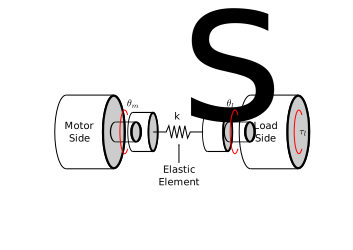
\includegraphics[width=0.7\textwidth]{Figures/Ch1/SEA.png}
    \caption{Rotary Style Series Elastic Actuator}
    \label{fig:SEA}
\end{figure}

The use of flexible components within robotic systems has been shown to be an effective way of improving performance metrics such as movement velocity and power efficiency \cite{Seok2015,Hurst2008}. Of the different techniques that have be deployed, the use of series elastic actuators (SEAs) has been shown to be effective \cite{Pratt1995,Ahmadi1997}. Storing energy in the non-rigid parts of motor joints, such as the elastic element seen in Figure~\ref{fig:SEA}, have proven to be an effective way for increasing efficiency. The addition of flexible joints is not the only technique that has been used to improve performance, however; utilizing tendon like elastic members to connect actuators to links has also been shown to be an effective way of improving efficiency \cite{Folkertsma2012}. The use of tendons, being an example of replicating what is found in nature, is a common method of finding unique mechanical designs that perform well in the real world. An example of this type of design can be seen in Figure~\ref{fig:tendon_leg}. Following a similar idea, research has also been conducted finding the usefulness of including flexibility in the spine of of 2D running robots, leading to dramatic increases in velocity \cite{Kani2013}. Research studying the effects of flexible links, like the ones shown in Figure~\ref{fig:flexible_system}, is limited though, particularly in the realm of legged-robots. Still, it has been shown as a viable method of increasing performance in these types of robots \cite{Horigomed}.
%
\begin{figure}[tb!]
  \centering
    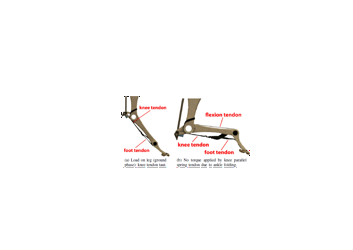
\includegraphics[width=0.75\textwidth]{Figures/Ch1/tendon_leg.png}
    \caption{Tendon Like Flexibility from \cite{Folkertsma2012}}
    \label{fig:tendon_leg}    
\end{figure}
% 

\section{Controlling Flexible Systems}
Control methods developed for flexible systems have been shown to be effective for position control and vibration reduction \cite{Luo1993, Ahmadi1997}. Due to the challenges seen in scaling the controllers to highly nonlinear systems, methods utilizing reinforcement learning are of interest. This method has been used in simple planar cases, where it was compared to a proportional-derivative (PD) control strategy for vibration suppression and proved to be a higher performing method \cite{He2020f}. Additionally, it has also been shown to be effective at defining control strategies for flexible-legged locomotion. The use of actor-critic algorithms such as Deep Deterministic Policy Gradient \cite{Lillicrap2016h} have been used to train running strategies for a flexible-legged quadruped \cite{Dwiel2019d}. Much of the research is based in simulation, however, and often the controllers are not deployed on physical systems, which leads to the question of whether or not these are useful techniques in practice. 

\section{Concurrent Design}
Defining an optimal controller for a system can be difficult due to challenges such as mechanical and electrical design limits. This is especially true when the system is flexible and the model is nonlinear. A solution to this challenge is to concurrently design a system with the controllers so that the two are jointly optimized. Defining the design process such that the design of the robot results in a simple dynamic model has been shown to improve the performance of mechatronics systems \cite{Li2001}. Additionally, in more recent work, the utilization of complex deep learning methods have shown to be an effective strategy for finding optimal concurrent designs \cite{Chen2020}. Deep learning has been used to find concurrent designs for simulated legged robotic systems, leading to improved performance in regards to movement velocity \cite{Schaff2019e}. Some research has even been completed where the designs were deployed on physical hardware, validating that this area of research is an effective one for learning how best to define system/controller architectures \cite{Whitman2020}. Little research exists utilizing these techniques on legged-robotic systems however, particularly ones with flexible components. 

\section{Reinforcement Learning}
\label{sec:rl}
With the recent successes seen in utilizing reinforcement learning (RL) to define control strategies, design parameters, and concurrent designs for robot systems, it is of interest to apply this technique in a unique way to flexible-legged jumping systems. Methods such as generative design have shown much success in being used to define mechanical designs, however most of this work is done wherein the information gathered from a system is done so in a static environment \cite{doi:10.1504/IJDE.2017.085639, briard:hal-02948764}. Reinforcement learning, in contrast, can be used to learn designs through dynamic environment interactions.

Reinforcement Learning is the process of training a policy to define a series of commands using an environment where those commands can be applied. This is an iterative process which is shown in Figure~\ref{fig:rl_process}. A policy, often referred to as an agent, from a controls theory perspective, is synonymous with a controller. The environment the controller is deployed in, again from a controls theory perspective, is synonymous with a robotic system. Training the controller requires iteratively deploying the controller's commands, or actions, to the environment and observing the results. The results are often in the form of the state of the environment and a reward resulting from the action that was applied. The reward function is defined by the designer so that the controller is trained to accomplish a desired task. Other than the reward, the controller has no way to discern what commands are good when the environment is in some state.
% 
\begin{figure}[tb!]
  \centering
    \includegraphics[width=0.5\textwidth]{Figures/Ch1/RL_Flow_Chart.drawio.png}
    \caption{Reinforcement Learning Process}
    \label{fig:rl_process}
\end{figure}
%

Learning an optimal control strategy is accomplished by deploying a gradient-decent-based learning algorithm utilizing information such as the state of the environment and the reward. For general robotics applications, at each discrete time step $t$, the environment will be in a state $s \in \mathcal{S}$, and the controller will select an action $a \in \mathcal{A}$ according to the current policy $\pi~:~\mathcal{S}~\rightarrow~\mathcal{A}$ and apply said action within the environment. The environment will transition to a new state $s'$ and will generate a reward $r$ based on the designer's definition of the reward function. The return, being the value the algorithm is trying to optimize, is defined as a discounted sum of rewards, $R_t = \sum_{i=t}^T \gamma^{i-t} \, r(s_i, a_i)$, where $\gamma$ is a discount factor for assigning the level of importance for near-term or long-term rewards.

The challenge of an RL algorithm is to optimize a policy, $\pi_{\phi}$, with parameters, $\phi$, such that actions generated at each time step will maximize the return. Ultimately, an optimized policy will maximize the expected return, $J(\phi) = \mathbb{E}_{s_i \thicksim p_{\pi}, a_i \thicksim \pi}[R_0]$. 
% Because many robotics controls processes are continuous control problems, the policy, $\pi_{\phi}$, can be updated using gradient decent in terms of the parameters $\phi$, which looks like $\nabla_{\phi} J(\phi)$. 

\section{Twin Delayed Deep Deterministic Policy Gradient}

There are many algorithms used to train a neural-network-based controller in an RL application, some of which have shown their ability to learn high-performing control strategies for robotic systems \cite{Zhao2020, Vecerik2017, Plappert2018}. Of the different algorithms used in current research, the one selected and tested in this work is Twin Delayed Deep Deterministic Policy Gradient (TD3) \cite{Fujimoto2018d}. This is an actor-critic learning algorithm which is widely considered the successor to the popular and proven Deep Deterministic Policy Gradient (DDPG) algorithm \cite{Lillicrap2016h}. 

\begin{sidewaysfigure}
  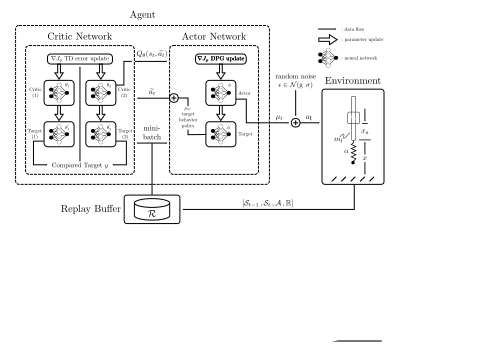
\includegraphics[width=\textwidth]{Figures/Ch1/TD3_Diagram.png}
  \caption{Twin Delayed Deep Deterministic Policy Gradient Block Diagram with Monopode as Environment}
  \label{fig:TD3}
\end{sidewaysfigure}

Figure~\ref{fig:TD3} displays the flow of information for this algorithm. In general, this algorithm learns both a Q-function and a policy, being the \textit{critic} and the \textit{actor}. For algorithms such as TD3, the ultimate goal is to find a policy, $\pi_{\theta}$, which maximizes the expected return:
% 
\begin{equation}
  \label{eq:expected_return}
  \begin{aligned}
    \nabla_{\phi} J(\phi) = \mathbb{E}_{s \thicksim p_{\pi}} \left [ \nabla_a Q^{\pi}(s,a)|_{a=\pi(s)} \nabla_{\phi}\pi_{\phi}(s) \right ]
  \end{aligned}
\end{equation}
%
where $Q^{\pi}(s,a) = \mathbb{E}_{s_i \thicksim p_{\pi}, a_i \thicksim \pi}[R_t|s,a]$ is the Q-function (sometimes called the value function) and the critic in the case of the TD3 architecture. This function is based on the Bellman Equation \cite{BellmanEquation} and returns a numerical value from being in a state $s$, taking action $a$, and following policy $\pi$ from there after:
% 
\begin{equation}
  \label{eq:bellman_eq}
  \begin{aligned}
    Q^{\pi}(s,a) = \underset{s' \thicksim P}{E} \left[ r(s,a) + \gamma \, \underset{a'}{\textup{max}} \, Q^{\pi}(s', a')  \right]
  \end{aligned}
\end{equation}
% 

Using a differentiable function approximator, $Q^{\pi}(s,a)$ can be represented and estimated by $Q_{\phi}(s,a)$, with parameters $\phi$ \cite{Mnihg}. Updating the Q-function is accomplished using the temporal difference error between the Q-function and a target Q-function \cite{Sutton1991, Watkins1989}. To maintain a fixed objective over multiple policy updates, the target Q-function approximator is instantiated separately as $Q_{\phi_{targ}}(s,a)$. The target does depend on the same parameters that are being trained, $\phi$, so there exists an issue when trying to use it as a target. To solve this issue the target network is updated at a delayed pace following the main Q-function approximator by either matching the parameters or by polyak averaging, $\phi_{targ} \leftarrow \tau \phi + (1-\tau)\phi_{targ}$, where $\tau$ is a tunable hyperparameter. 

In summary, the critic side of the TD3 algorithm is responsible for minimizing the difference between the value of the current state/action pair using the main Q-function, and the reward of the current state/action pair plus the discounted value of the next state/action pair using the target Q-function. The loss function takes the form:
% 
\begin{equation}
  \label{eq:q_func_loss}
  \begin{aligned}
    L(\phi, \mathcal{D}) = \underset{(s,a,r,s',d) \thicksim \mathcal{D}}{E} \left[ \left( Q_{\phi}(s,a) - \left( r(s,a) + \gamma \, (1-d) \, Q_{\phi_{targ}}(s', \pi_{\theta_{targ}}(s')) \right)  \right)^2 \right]
  \end{aligned}
\end{equation}
% 
where $\pi_{\theta_{targ}}(s')$ is a target policy that, in a similar manner to the target Q-function, follows the main policy, $\pi_{\theta}$, at a delayed pace either by directly copying the values or by Polyak averaging. Additionally, $d$ represents a boolean value which depends on the terminal status of the next state, $s'$. 

As for updating the policy for the actor critic-type algorithm, this aspect is rather simple. Because DDPG, and therefore TD3, are built to accommodate only continuous action spaces, the Q-function is assumed to be differentiable with respect to action. Therefore, to find optimal policy parameters, $\theta$, for the policy, $\pi_{\theta}$, the solution of the Q function must be found:
% 
\begin{equation}
  \label{eq:policy_update}
  \begin{aligned}
    \underset{\theta}{\textup{max}} \, \underset{s \thicksim \mathcal{D}}{E} \, \left[Q_{\phi}(s, \pi_{\theta}(s))\right]
  \end{aligned}
\end{equation}

The reason that TD3 is considered the successor to DDPG is that there are some additional tricks deployed in addition to the description thus far. The first is the addition of noise to the target policy. It can be seen in~(\ref{eq:q_func_loss}) that the target policy, $\pi_{\theta_{targ}}$, is required to generate an action to evaluate the target Q-function. Noise is added to the policy, taking the form:
% 
\begin{equation}
  \label{eq:action_noise}
  \begin{aligned}
    a'(s') = \textup{clip} \, \left( \pi_{\theta_{targ}}(s') + \textup{clip}(\epsilon, -c, c), a_{low}, a_{high}  \right), ~~~ \epsilon \thicksim \mathcal{N}(0,\sigma)
  \end{aligned}
\end{equation}
% 
where $\epsilon$ represents the noise sampled using some user specified method. This method of adding noise was shown to reduce the issue of the Q-function approximator developing large values for certain state/action pairs, therefore smoothing the Q-function. 

The second trick the TD3 algorithm employs is the addition of a second Q-function approximator and target Q-function approximator. A known potential issue of the Q-function is that it can suffer from overestimation of the value of action/state pairs. This, of course, leads to the policy learning actions that the Q-function assumes are better than they actually are. To alleviate this issue, two Q-functions and two target Q-functions are instantiated. Calculating the target Q-function is then completed by evaluating the two target Q-functions:
% 
\begin{equation}
  \begin{aligned}
    y(r,s',d) = r(s,a) + \gamma \, (1-d) \, Q_{\phi_{i,targ}}(s', \pi_{\theta_{targ}}(s')),~~~ \textup{for}~i=1,2
  \end{aligned}
\end{equation}
% 
and taking the lower of the two targets to update both the main Q-functions:
% 
\begin{equation}
  \begin{aligned}
    L(\phi_1, \mathcal{D}) = \underset{(s,a,r,s',d) \thicksim \mathcal{D}}{E} \left[ \left( Q_{\phi_1}(s,a) - y(r,s',d) \right)^2 \right]
  \end{aligned}
\end{equation}
% 
\begin{equation}
  \begin{aligned}
    L(\phi_2, \mathcal{D}) = \underset{(s,a,r,s',d) \thicksim \mathcal{D}}{E} \left[ \left( Q_{\phi_2}(s,a) - y(r,s',d) \right)^2 \right]
  \end{aligned}
\end{equation}.
% 

The last technique that the TD3 algorithm employs is the addition of a delay between to the policy update in regards to the Q-function update. It has been shown that in doing this the Q-function is able to converge to a better solution before updating the policy. Ultimately, the addition of a policy update delay was utilized to reduce coupling between the Q-function and the policy. The recommended delay is updating the policy every two Q-function updates.

There are many implementations of the TD3 algorithm that are publicly available. Of these, the \textbf{\textbf{StableBaselines3}} implementation is used to complete the work in this thesis \cite{stable-baselines3}. \textbf{\textbf{StableBaselines3}} is a widely used library of RL algorithm implementations and is composed of well written and understandable documentation for the supported implementations. The differentiable function approximators used to estimate the policies and Q-functions are built within \textbf{StableBaselines3} using PyTorch \cite{NEURIPS2019_9015}, which is also a widely used framework for machine learning and more specifically reinforcement learning. 

\section{Contributions}

The purpose of the work presented in the remainder of this thesis is to propose and evaluate the performance of a concurrent design architecture that utilizes RL techniques for flexible jumping systems. A concurrent design system in this work is one that concurrently learns a mechanical/electrical design for a system and an associated control policy for said system. There is an absence of literature surrounding RL-based concurrent design, particularly regarding locomotive robotics applications. Therefore, in this work, an RL-based method is proposed that seeks to learn better performing designs than ones that implement isolated mechanical/electrical and controller policy design. The method will be evaluated in simulation on a simplified flexible-legged jumping monopode where better designs are ones that jump higher and perform more efficiently. The components which build the concurrent design architecture will be split across the next few chapters wherein additional findings will be presented.

In the next chapter, a RL-based controller will be trained on a monopode jumping system to evaluate the effectiveness of training for efficient control. Power use is often considered when designing RL controllers for rigid systems, typically taking the form of a weighted negative reward when deploying an RL algorithm. It will be evaluated by defining strategies for flexible systems, where efficiency is the primary objective, if the resulting control strategy takes advantage of system flexibility. To determine if the learned policies are approaching what current literature supports regarding optimal control, the performance will be evaluated against input shaping techniques in Chapter~\ref{chapter3}.

Additionally, the need arises for incorporating mechanical design parameters into the learning process. Therefore, in Chapter~\ref{chapter4}, an RL problem is defined in a unique way such that the environment the RL policy is deployed in is a simulation of an environment where the actions sent by the policy are mechanical design updates. The method will be evaluated on the monopode jumping system to learn mechanical design parameters related to flexibility. Futhermore, using a single, fixed control input, it is of interest to determine if this technique can be used to define designs to accomplish multiple tasks. Therefore, using a single control input generated from the aforementioned input shaping techniques, the RL learning method will be tested for learning designs that cause the monopode to jump to multiple heights.

Next, in Chapter~\ref{chapter5}, the methods of learning a control policy and a design will be combined to create a concurrent design architecture. Two methods of implementing the mechanical design update will be shown, and the effects of the two methods will be discussed. Furthermore, a newly introduced hyperparameter when implementing the constructed concurrent design will be evaluated and the results will be discussed. The methods will be tested to compare efficient jumping and non-efficient jumping concurrent designs for the monopode jumping system. Ultimately, the resulting concurrent design performance will be presented and compared to the performance of control policies trained on static designs.

Lastly, in Chapter~\ref{chapter6}, the work presented in this thesis will be summarized and the results of the proposed concurrent design process will be highlighted. Accompanying the conclusive remarks, future research that has been enabled by the work presented will be discussed, along with recommended next steps for starting this future work.  